\documentclass[12pt]{article}
\usepackage{ifluatex}\ifluatex
\ifx\pdfpagewidth\undefined\let\pdfpagewidth\paperwidth\fi
\ifx\pdfpageheight\undefined\let\pdfpageheight\paperheight\fi\else
\let\paperwidthsave\paperwidth\let\paperwidth\undefined
\usepackage{graphicx}
\let\paperwidth\paperwidthsave\fi
\newbox\ASYbox
\newdimen\ASYdimen
\def\ASYprefix{}
\long\def\ASYbase#1#2{\leavevmode\setbox\ASYbox=\hbox{#1}%\ASYdimen=\ht\ASYbox%
\setbox\ASYbox=\hbox{#2}\lower\ASYdimen\box\ASYbox}
\long\def\ASYaligned(#1,#2)(#3,#4)#5#6#7{\leavevmode%
\setbox\ASYbox=\hbox{#7}%
\setbox\ASYbox\hbox{\ASYdimen=\ht\ASYbox%
\advance\ASYdimen by\dp\ASYbox\kern#3\wd\ASYbox\raise#4\ASYdimen\box\ASYbox}%
\setbox\ASYbox=\hbox{#5\wd\ASYbox 0pt\dp\ASYbox 0pt\ht\ASYbox 0pt\box\ASYbox#6}%
\hbox to 0pt{\kern#1pt\raise#2pt\box\ASYbox\hss}}%
\long\def\ASYalignT(#1,#2)(#3,#4)#5#6{%
\ASYaligned(#1,#2)(#3,#4){%
\special{pdf:q #5 0 0 cm}%
}{%
\special{pdf:Q}%
}{#6}}
\long\def\ASYalign(#1,#2)(#3,#4)#5{\ASYaligned(#1,#2)(#3,#4){}{}{#5}}
\def\ASYraw#1{#1}
\usepackage{graphicx}
\usepackage{color}
\pdfpagewidth=137.062992bp
\ifx\pdfhorigin\undefined
\hoffset=-1in
\voffset=-72.000000bp
\pdfpageheight=137.062992bp
\else
\pdfhorigin=0bp
\pdfvorigin=0.000000bp
\pdfpageheight=137.062992bp
\fi
\setlength{\unitlength}{1pt}
\pagestyle{empty}
\textheight=155.062992bp
\textwidth=155.062992bp
\oddsidemargin=-17.61pt
\evensidemargin=\oddsidemargin
\topmargin=-37.01pt
\begin{document}
\makeatletter%
\let\ASYencoding\f@encoding%
\let\ASYfamily\f@family%
\let\ASYseries\f@series%
\let\ASYshape\f@shape%
\makeatother%
{\catcode`"=12%
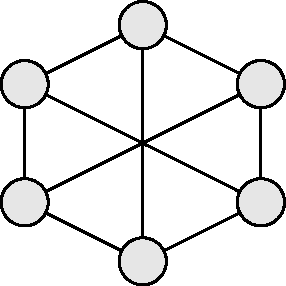
\includegraphics{figure-2-4_0.pdf}%
}%
\kern -137.576978pt%
\definecolor{ASYcolor}{gray}{0.000000}\color{ASYcolor}
\fontsize{12.000000}{14.400000}\selectfont
\usefont{\ASYencoding}{\ASYfamily}{\ASYseries}{\ASYshape}%
\ASYalign(11.882977,97.241245)(-0.500000,-0.500000){0}%
\definecolor{ASYcolor}{gray}{0.000000}\color{ASYcolor}
\fontsize{12.000000}{14.400000}\selectfont
\ASYalign(68.788489,11.882977)(-0.500000,-0.500000){1}%
\definecolor{ASYcolor}{gray}{0.000000}\color{ASYcolor}
\fontsize{12.000000}{14.400000}\selectfont
\ASYalign(125.694001,40.335733)(-0.500000,-0.500000){2}%
\definecolor{ASYcolor}{gray}{0.000000}\color{ASYcolor}
\fontsize{12.000000}{14.400000}\selectfont
\ASYalign(68.788489,125.694001)(-0.500000,-0.500000){3}%
\definecolor{ASYcolor}{gray}{0.000000}\color{ASYcolor}
\fontsize{12.000000}{14.400000}\selectfont
\ASYalign(11.882977,40.335733)(-0.500000,-0.500000){4}%
\definecolor{ASYcolor}{gray}{0.000000}\color{ASYcolor}
\fontsize{12.000000}{14.400000}\selectfont
\ASYalign(125.694001,97.241245)(-0.500000,-0.500000){5}%
\definecolor{ASYcolor}{gray}{0.000000}\color{ASYcolor}
\fontsize{12.000000}{14.400000}\selectfont
\definecolor{ASYcolor}{gray}{0.000000}\color{ASYcolor}
\fontsize{12.000000}{14.400000}\selectfont
\definecolor{ASYcolor}{gray}{0.000000}\color{ASYcolor}
\fontsize{12.000000}{14.400000}\selectfont
\definecolor{ASYcolor}{gray}{0.000000}\color{ASYcolor}
\fontsize{12.000000}{14.400000}\selectfont
\definecolor{ASYcolor}{gray}{0.000000}\color{ASYcolor}
\fontsize{12.000000}{14.400000}\selectfont
\definecolor{ASYcolor}{gray}{0.000000}\color{ASYcolor}
\fontsize{12.000000}{14.400000}\selectfont
\definecolor{ASYcolor}{gray}{0.000000}\color{ASYcolor}
\fontsize{12.000000}{14.400000}\selectfont
\definecolor{ASYcolor}{gray}{0.000000}\color{ASYcolor}
\fontsize{12.000000}{14.400000}\selectfont
\definecolor{ASYcolor}{gray}{0.000000}\color{ASYcolor}
\fontsize{12.000000}{14.400000}\selectfont
\end{document}
